
	\RequirePackage{fix-cm}
	%Journal of Mathematical Imaging and Vision
	\documentclass[twocolumn]{svjour3}
	
	
	\smartqed  % flush right qed marks, e.g. at end of proof
	
	\usepackage{times}
	\usepackage{bm,bbm}
	\usepackage{amsmath,amssymb}
	\usepackage{graphicx,subfigure}
	\usepackage{url}
	\usepackage{units}
	\usepackage{cite,balance}
	\usepackage{comment}
	\usepackage{multirow}
	\usepackage{booktabs}
	\usepackage{microtype}
	\usepackage{siunitx}
	\usepackage{color}
	\usepackage{float}
	%\usepackage{auto-pst-pdf}
	\usepackage{wrapfig}
	
	\usepackage{mathptmx}
	
	\usepackage{array}
	\usepackage{varwidth}
	
	
	\usepackage[normalem]{ulem} %%%% para tachar texto
	
	%-----------------------
	%Bibliography style
	%\usepackage[numbers]{natbib}
	
	%\newtheorem{definition}{Definition}
	%\newtheorem{proposition}{Proposition}
	\newcommand{\at}[2][]{#1|_{#2}}
	%\newcommand{\K}{\text{K}}
	
	\newcommand{\mc}[1]{\multicolumn{1}{c}{#1}}
	\newcommand{\argmin}{\operatorname*{\text{arg min }}}
	
	%\ifpdf
	%\graphicspath{{/Users/acfrery/Documents/Alunos/Julia Cassetti/Figures/PaperTesis}{/Users/acfrery/Documents/Alunos/Julia Cassetti/Figures/PaperTesis/ConModificacionAlejandro}{/Users/acfrery/Documents/Alunos/Julia Cassetti/Figures/PaperTesis/Viejos}}
	%\else
	%\graphicspath{{/Users/acfrery/Documents/Alunos/Julia Cassetti/Figures/PaperTesis}{/Users/acfrery/Documents/Alunos/Julia Cassetti/Figures/PaperTesis/ConModificacionAlejandro}{/Users/acfrery/Documents/Alunos/Julia Cassetti/Figures/PaperTesis/Viejos}}
	%\fi
	
	\begin{document}
	\begin{wrapfigure}{l}{28mm} 
		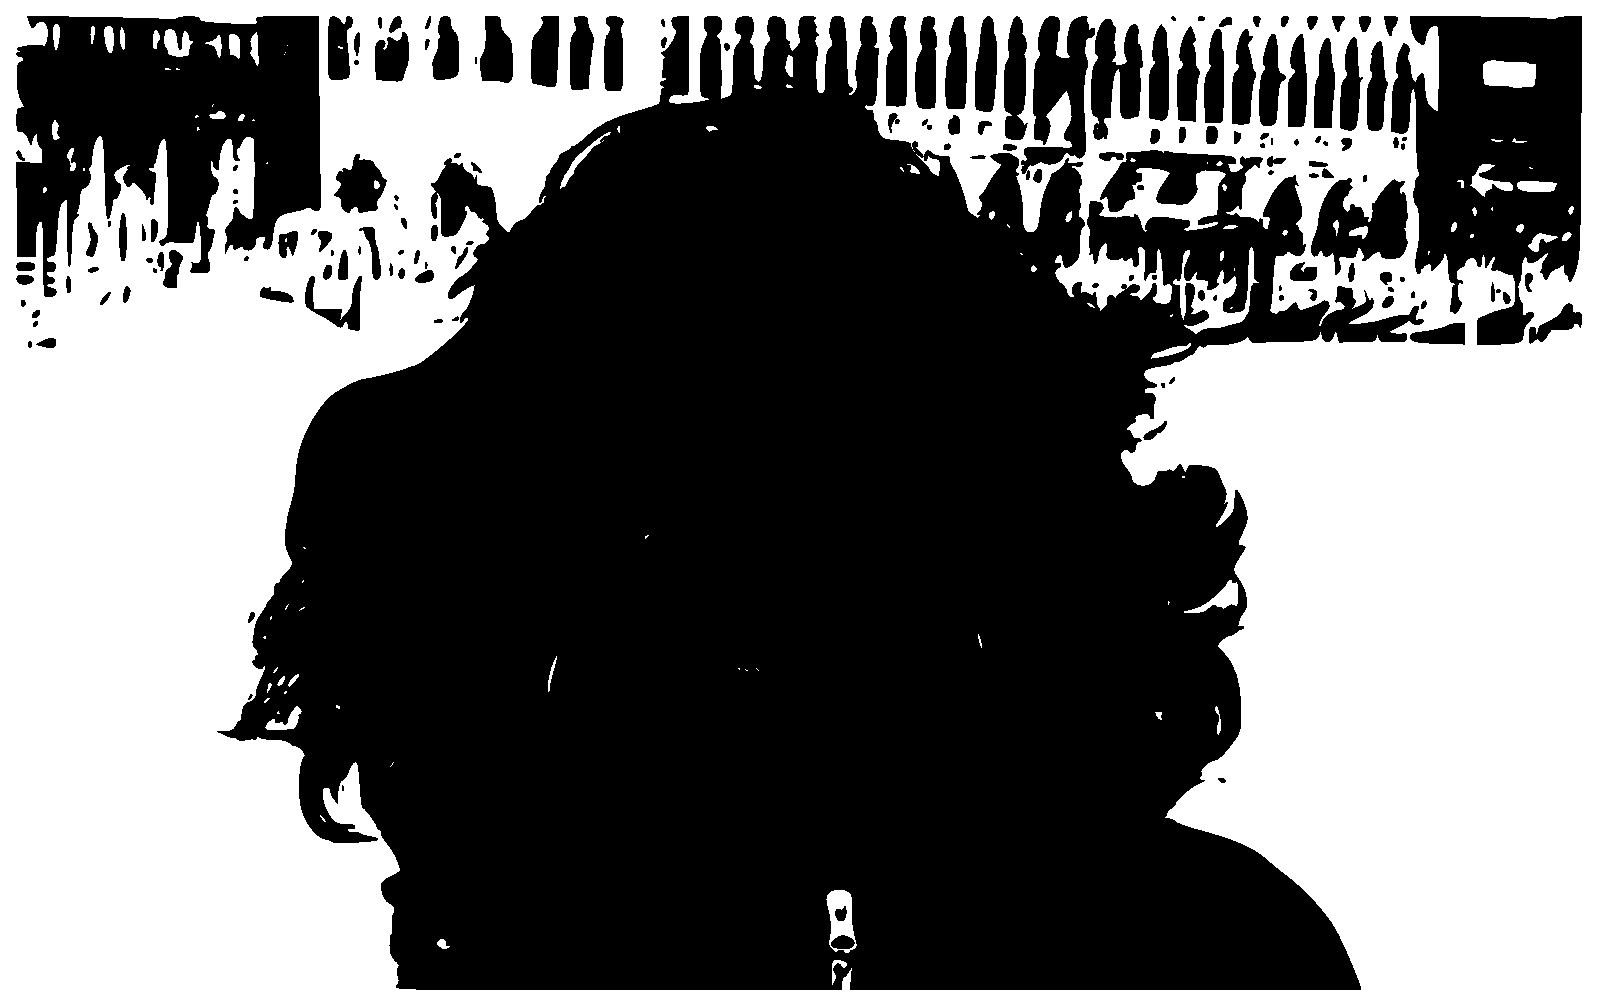
\includegraphics[width=1.1in,height=1.3in,clip]{Cassetti}
	\end{wrapfigure}\par
	\textbf{Julia Cassetti} received the B.Sc. degree in Mathematics and a postgraduate diploma in Mathematical Statistics, both from the Universidad de Buenos Aires (UBA), Argentina. Her Ph.D. degree was in Ciencie from the Universidad Nacional de General Sarmiento, Argentina. She is currently a Professor at the Universidad Nacional de General Sarmiento, Argentina. Her research interests are SAR imaging and applied statistics and statistical computing.\par
	
	
	\begin{wrapfigure}{l}{25mm} 
		\includegraphics[width=1in,height=2in,clip,keepaspectratio]{Frery}
	\end{wrapfigure}\par
	\textbf{Alejandro C. Frery} received a B.Sc. degree in Electronic and Electrical Engineering from the Universidad de Mendoza, Mendoza, Argentina.
	His M.Sc. degree was in Applied Mathematics (Statistics) from the Instituto de Matem\'atica Pura e Aplicada (IMPA, Rio de Janeiro) and his Ph.D. degree was in Applied Computing from the Instituto Nacional de Pesquisas Espaciais (INPE, S\~ao Jos\'e dos Campos, Brazil).
	He is Professor with the School of Mathematics and Statistics, Victoria University of Wellington, New Zealand.
	His research interests are statistical computing and stochastic modeling.
	\par
	
	\end{document}
	